\begin{tikzpicture}
    % ---------------------------------------------------------
    \node[rotate=90] at (-5.3, 0) {\begin{tabular}{c}{\bf (1) Shape Prior}\\[1mm]{\small Variational}\\ {\small Auto-Encoder \cite{Kingma2014ICLR}}\end{tabular}};
    
    \node[rectangle,draw=black,anchor=west] (prior) at (-4.5,0) {
        \begin{tabular}{c}
	        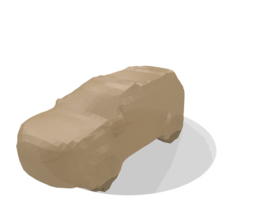
\includegraphics[height=1cm,trim={\cropleft cm \croplower cm \cropright cm \cropupper cm},clip]{overview_large/00010_target_off}
	        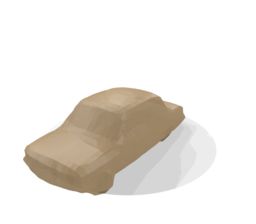
\includegraphics[height=1cm,trim={\cropleft cm \croplower cm \cropright cm \cropupper cm},clip]{overview_large/00004_target_off}\\
	        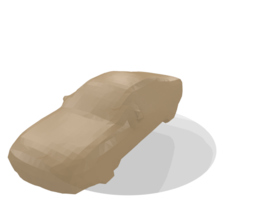
\includegraphics[height=1cm,trim={\cropleft cm \croplower cm \cropright cm \cropupper cm},clip]{overview_large/00000_target_off}
	        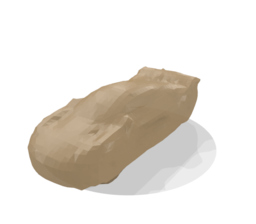
\includegraphics[height=1cm,trim={\cropleft cm \croplower cm \cropright cm \cropupper cm},clip]{overview_large/00012_target_off}
        \end{tabular}
    };
    \node[anchor=south] at ($(prior.north) + (0,0.05)$) {Synthetic Training Data};
    
    \node[] (y) at (0, 1.5) {Shape $y$};
    
    \node[rectangle,draw=black,anchor=west] (input) at (-1, 0) {
        \begin{tabular}{c}
            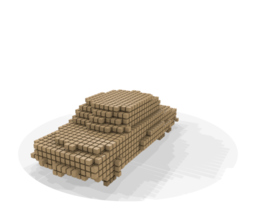
\includegraphics[height=1cm,trim={\cropleft cm \croplower cm \cropright cm \cropupper cm},clip]{overview_large/00004_target_binvox}\\
            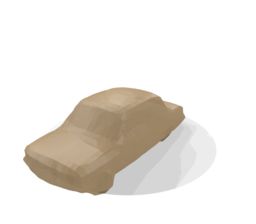
\includegraphics[height=1cm,trim={\cropleft cm \croplower cm \cropright cm \cropupper cm},clip]{overview_large/00004_target_off}
        \end{tabular}
    };
  
    \draw ($(input.north east) + (0.2,0)$) -- ($(input.north east) + (1.5,-0.75)$) -- ($(input.north east) + (1.5,-1.75)$) -- ($(input.south east) + (0.2,0)$) -- ($(input.north east) + (0.2,0)$);
    \node at ($(input.east) + (0.825,0)$) {\small encoder};
    
    \node (z) at (2.75, 0) {$z$};
    
    \node[rectangle,draw=black,anchor=east] (output) at (6.5, 0) {
        \begin{tabular}{c}
        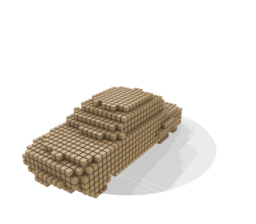
\includegraphics[height=1cm,trim={\cropleft cm \croplower cm \cropright cm \cropupper cm},clip]{overview_large/00004_prediction_binvox}\\
        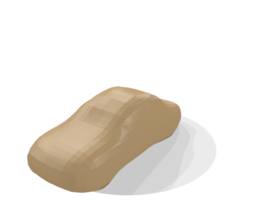
\includegraphics[height=1cm,trim={\cropleft cm \croplower cm \cropright cm \cropupper cm},clip]{overview_large/00004_prediction_off}
        \end{tabular}
    };
    
    \draw ($(output.north west) - (0.2,0)$) -- ($(output.north west) - (1.5,0.75)$) -- ($(output.north west) - (1.5,1.75)$) -- ($(output.south west) - (0.2,0)$) -- ($(output.north west) - (0.2,0)$);
    \node at ($(output.west) - (0.825,0)$) {\small decoder};
    
    \node (ry) at (5.5, 1.5) {Rec. Shape $\tilde{y}$};
    
    \node[] (L) at (2.75, 1.9) {Reconstruction Loss};
    
    \draw[-] (ry) -- ($(ry) + (0,0.4)$);
    \draw[-] ($(ry) + (0,0.4)$) -- (L);
    \draw[-] (y) -- ($(y) + (0,0.4)$);
    \draw[-] ($(y) + (0,0.4)$) -- (L);    
    
    \begin{scope}[shift={(0,-4)}]
    
	    % ---------------------------------------------------------
	    \node[rotate=90] at (-5.3, 0) {\begin{tabular}{c}{\bf(2) Shape Inference}\\[1mm]{\small Amortized}\\{\small Maximum Likelihood}\end{tabular}};
	    
	    \node[rectangle,draw=black,anchor=west] (inference) at (-4.5,0) {
	        \begin{tabular}{c}
		        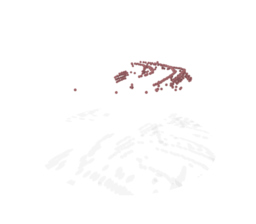
\includegraphics[height=1cm,trim={\cropleft cm \croplower cm \cropright cm \cropupper cm},clip]{overview_large/00037_input_txt}
		        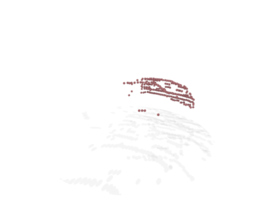
\includegraphics[height=1cm,trim={\cropleft cm \croplower cm \cropright cm \cropupper cm},clip]{overview_large/00005_input_txt}
		        \\
		        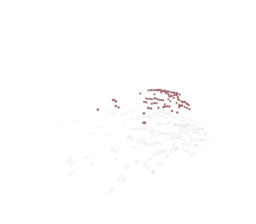
\includegraphics[height=1cm,trim={\cropleft cm \croplower cm \cropright cm \cropupper cm},clip]{overview_large/00045_input_txt}
		        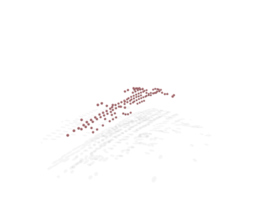
\includegraphics[height=1cm,trim={\cropleft cm \croplower cm \cropright cm \cropupper cm},clip]{overview_large/00047_input_txt}
	        \end{tabular}
	    };
	    
	    \node[anchor=north] at ($(inference.south) - (0,0.05)$) {\begin{tabular}{c}Real Training Data\\w/o Targets\end{tabular}};
	    
	    % --
	    \node(correspondence) at ($(inference) + (0,2)$) {\small\textbf{no correspondence needed}};
	    \draw[-,dotted] (prior) -- (correspondence);
	    \draw[-,dotted] (correspondence) -- (inference);
	    
	    \node(retain) at ($(correspondence) + (7,0)$) {retain fixed decoder};
	    \draw[-] ($(prior) + (7,-1.15)$) -- (retain);
	    \draw[->] (retain) -- ($(inference) + (7,1.15)$);
	    
	    \node[] (y) at (0, -1.5) {Observation $x$};
	    
	    \node[rectangle,draw=black,anchor=west] (input) at (-1, 0) {
	        \begin{tabular}{c}
	        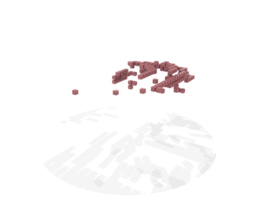
\includegraphics[height=1cm,trim={\cropleft cm \croplower cm \cropright cm \cropupper cm},clip]{overview_large/00037_input_binvox}\\
	        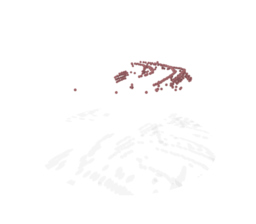
\includegraphics[height=1cm,trim={\cropleft cm \croplower cm \cropright cm \cropupper cm},clip]{overview_large/00037_input_txt}
	        \end{tabular}
	    };
	    
	    \draw ($(input.north east) + (0.2,0)$) -- ($(input.north east) + (1.5,-0.75)$) -- ($(input.north east) + (1.5,-1.75)$) -- ($(input.south east) + (0.2,0)$) -- ($(input.north east) + (0.2,0)$);
        \node at ($(input.east) + (0.825,0)$) {\small encoder};
	    
	    \node (z) at (2.75, 0) {$z$};
	    
	    \node[rectangle,draw=black,anchor=east] (output) at (6.5, 0) {
	        \begin{tabular}{c}
	        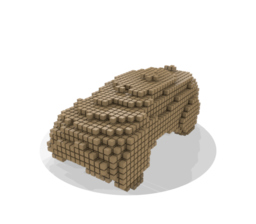
\includegraphics[height=1cm,trim={\cropleft cm \croplower cm \cropright cm \cropupper cm},clip]{overview_large/00037_prediction_binvox}\\
	        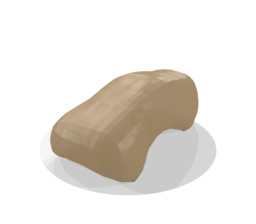
\includegraphics[height=1cm,trim={\cropleft cm \croplower cm \cropright cm \cropupper cm},clip]{overview_large/00037_prediction_off}
	        \end{tabular}
	    };
	    
	    \draw ($(output.north west) - (0.2,0)$) -- ($(output.north west) - (1.5,0.75)$) -- ($(output.north west) - (1.5,1.75)$) -- ($(output.south west) - (0.2,0)$) -- ($(output.north west) - (0.2,0)$);
	    \node at ($(output.west) - (0.825,0)$) {\small decoder};
	    
	    \node (ry) at (5.5, -1.5) {Prop. Shape $\tilde{y}$};
	    
	    \node[] (L) at (2.75, -2.1) {\begin{tabular}{c}Unsupervised\\Maximum Likelihood Loss\end{tabular}};
	    
	    \draw[-] (ry) -- ($(ry) - (0,0.6)$);
	    \draw[-] ($(ry) - (0,0.6)$) -- (L);
	    \draw[-] (y) -- ($(y) - (0,0.6)$);
	    \draw[-] ($(y) - (0,0.6)$) -- (L);
    \end{scope}
\end{tikzpicture}
